% ****************************************************************************************
% *****************          EJERCICIO DE ALGORITMOS           ***************************
% ****************************************************************************************


% =======================================================
% =======         HEADER FOR DOCUMENT        ============
% =======================================================
    
    % *********   HEADERS AND FOOTERS ********
    \def\ProjectAuthorLink{https://github.com/SoyOscarRH}           %Just to keep it in line
    \def\ProjectNameLink{\ProjectAuthorLink/Proyect}                %Link to Proyect

    % *********   DOCUMENT ITSELF   **************
    \documentclass[12pt, fleqn]{article}                            %Type of document and size of font
    \usepackage[spanish]{babel}                                     %Please use spanish
    \usepackage[utf8]{inputenc}                                     %Please use spanish - UFT
    \usepackage[margin = 1.2in]{geometry}                           %Margins and Geometry pacakge
    \usepackage{ifthen}                                             %Allow simple programming
    \usepackage{hyperref}                                           %Create MetaData for a PDF and LINKS!
    \usepackage{pdfpages}                                           %Create MetaData for a PDF and LINKS!
    \hypersetup{pageanchor = false}                                 %Solve 'double page 1' warnings in build
    \setlength{\parindent}{0pt}                                     %Eliminate ugly indentation
    \author{Oscar Andrés Rosas}                                     %Who I am

    % *********   LANGUAJE    *****************
    \usepackage[T1]{fontenc}                                        %Please use spanish
    \usepackage{textcmds}                                           %Allow us to use quoutes
    \usepackage{changepage}                                         %Allow us to use identate paragraphs
    \usepackage{anyfontsize}                                        %All the sizes

    % *********   MATH AND HIS STYLE  *********
    \usepackage{ntheorem, amsmath, amssymb, amsfonts}               %All fucking math, I want all!
    \usepackage{mathrsfs, mathtools, empheq}                        %All fucking math, I want all!
    \usepackage{cancel}                                             %Negate symbol
    \usepackage{centernot}                                          %Allow me to negate a symbol
    \decimalpoint                                                   %Use decimal point

    % *********   GRAPHICS AND IMAGES *********
    \usepackage{graphicx}                                           %Allow to create graphics
    \usepackage{float}                                              %For images
    \usepackage{wrapfig}                                            %Allow to create images
    \graphicspath{ {Graphics/} }                                    %Where are the images :D

    % *********   LISTS AND TABLES ***********
    \usepackage{listings, listingsutf8}                             %We will be using code here
    \usepackage[inline]{enumitem}                                   %We will need to enumarate
    \usepackage{tasks}                                              %Horizontal lists
    \usepackage{longtable}                                          %Lets make tables awesome
    \usepackage{booktabs}                                           %Lets make tables awesome
    \usepackage{tabularx}                                           %Lets make tables awesome
    \usepackage{multirow}                                           %Lets make tables awesome
    \usepackage{multicol}                                           %Create multicolumns

    % *********   HEADERS AND FOOTERS ********
    \usepackage{fancyhdr}                                           %Lets make awesome headers/footers
    \pagestyle{fancy}                                               %Lets make awesome headers/footers
    \setlength{\headheight}{16pt}                                   %Top line
    \setlength{\parskip}{0.5em}                                     %Top line
    \renewcommand{\footrulewidth}{0.5pt}                            %Bottom line

    \lhead {                                                        %Left Header
        \hyperlink{section.\arabic{section}}                        %Make a link to the current chapter
        {\normalsize{\textsc{\nouppercase{\leftmark}}}}             %And fot it put the name
    }

    \rhead {                                                        %Right Header
        \hyperlink{section.\arabic{section}.\arabic{subsection}}    %Make a link to the current chapter
            {\footnotesize{\textsc{\nouppercase{\rightmark}}}}      %And fot it put the name
    }

    \rfoot{\textsc{\small{\hyperref[sec:Index]{Ve al Índice}}}}     %This will always be a footer  

    \fancyfoot[L]{                                                  %Algoritm for a changing footer
        \ifthenelse{\isodd{\value{page}}}                           %IF ODD PAGE:
            {\href{https://compilandoconocimiento.com/nosotros/}    %DO THIS:
                {\footnotesize                                      %Send the page
                    {\textsc{Oscar Andrés Rosas}}}}                 %Send the page
            {\href{https://compilandoconocimiento.com}              %ELSE DO THIS: 
                {\footnotesize                                      %Send the author
                    {\textsc{Compilando Conocimiento}}}}            %Send the author
    }
    
    
    
% =======================================================
% ===================   COMMANDS    =====================
% =======================================================

    % =========================================
    % =======   NEW ENVIRONMENTS   ============
    % =========================================
    \newenvironment{Indentation}[1][0.75em]                         %Use: \begin{Inde...}[Num]...\end{Inde...}
        {\begin{adjustwidth}{#1}{}}                                 %If you dont put nothing i will use 0.75 em
        {\end{adjustwidth}}                                         %This indentate a paragraph
    \newenvironment{SmallIndentation}[1][0.75em]                    %Use: The same that we upper one, just 
        {\begin{adjustwidth}{#1}{}\begin{footnotesize}}             %footnotesize size of letter by default
        {\end{footnotesize}\end{adjustwidth}}                       %that's it

    \newenvironment{MultiLineEquation}[1]                           %Use: To create MultiLine equations
        {\begin{equation}\begin{alignedat}{#1}}                     %Use: \begin{Multi..}{Num. de Columnas}
        {\end{alignedat}\end{equation}}                             %And.. that's it!
    \newenvironment{MultiLineEquation*}[1]                          %Use: To create MultiLine equations
        {\begin{equation*}\begin{alignedat}{#1}}                    %Use: \begin{Multi..}{Num. de Columnas}
        {\end{alignedat}\end{equation*}}                            %And.. that's it!
    

    % =========================================
    % == GENERAL TEXT & SYMBOLS ENVIRONMENTS ==
    % =========================================
    
    % =====  TEXT  ======================
    \newcommand \Quote {\qq}                                        %Use: \Quote to use quotes
    \newcommand \Over {\overline}                                   %Use: \Bar to use just for short
    \newcommand \ForceNewLine {$\Space$\\}                          %Use it in theorems for example

    % =====  SPACES  ====================
    \DeclareMathOperator \Space {\quad}                             %Use: \Space for a cool mega space
    \DeclareMathOperator \MegaSpace {\quad \quad}                   %Use: \MegaSpace for a cool mega mega space
    \DeclareMathOperator \MiniSpace {\;}                            %Use: \Space for a cool mini space
    
    % =====  MATH TEXT  =================
    \newcommand \Such {\MiniSpace | \MiniSpace}                     %Use: \Such like in sets
    \newcommand \Also {\MiniSpace \text{y} \MiniSpace}              %Use: \Also so it's look cool
    \newcommand \Remember[1]{\Space\text{\scriptsize{#1}}}          %Use: \Remember so it's look cool
    
    % =====  THEOREMS  ==================
    \newtheorem{Theorem}{Teorema}[section]                          %Use: \begin{Theorem}[Name]\label{Nombre}...
    \newtheorem{Corollary}{Colorario}[Theorem]                      %Use: \begin{Corollary}[Name]\label{Nombre}...
    \newtheorem{Lemma}[Theorem]{Lemma}                              %Use: \begin{Lemma}[Name]\label{Nombre}...
    \newtheorem{Definition}{Definición}[section]                    %Use: \begin{Definition}[Name]\label{Nombre}...
    \theoremstyle{break}                                            %THEOREMS START 1 SPACE AFTER

    % =====  LOGIC  =====================
    \newcommand \lIff    {\leftrightarrow}                          %Use: \lIff for logic iff
    \newcommand \lEqual  {\MiniSpace \Leftrightarrow \MiniSpace}    %Use: \lEqual for a logic double arrow
    \newcommand \lInfire {\MiniSpace \Rightarrow \MiniSpace}        %Use: \lInfire for a logic infire
    \newcommand \lLongTo {\longrightarrow}                          %Use: \lLongTo for a long arrow

    % =====  FAMOUS SETS  ===============
    \DeclareMathOperator \Naturals     {\mathbb{N}}                 %Use: \Naturals por Notation
    \DeclareMathOperator \Primes       {\mathbb{P}}                 %Use: \Primes por Notation
    \DeclareMathOperator \Integers     {\mathbb{Z}}                 %Use: \Integers por Notation
    \DeclareMathOperator \Racionals    {\mathbb{Q}}                 %Use: \Racionals por Notation
    \DeclareMathOperator \Reals        {\mathbb{R}}                 %Use: \Reals por Notation
    \DeclareMathOperator \Complexs     {\mathbb{C}}                 %Use: \Complex por Notation
    \DeclareMathOperator \GenericField {\mathbb{F}}                 %Use: \GenericField por Notation
    \DeclareMathOperator \VectorSet    {\mathbb{V}}                 %Use: \VectorSet por Notation
    \DeclareMathOperator \SubVectorSet {\mathbb{W}}                 %Use: \SubVectorSet por Notation
    \DeclareMathOperator \Polynomials  {\mathbb{P}}                 %Use: \Polynomials por Notation
    \DeclareMathOperator \VectorSpace  {\VectorSet_{\GenericField}} %Use: \VectorSpace por Notation
    \DeclareMathOperator \LinealTransformation {\mathcal{T}}        %Use: \LinealTransformation for a cool T
    \DeclareMathOperator \LinTrans {\mathcal{T}}                    %Use: \LinTrans for a cool T


    % =====  CONTAINERS   ===============
    \newcommand{\Set}[1]    {\left\{ \; #1 \; \right\}}             %Use: \Set {Info} for INTELLIGENT space 
    \newcommand{\bigSet}[1] {\big\{  \; #1 \; \big\}}               %Use: \bigSet  {Info} for space 
    \newcommand{\BigSet}[1] {\Big\{  \; #1 \; \Big\}}               %Use: \BigSet  {Info} for space 
    \newcommand{\biggSet}[1]{\bigg\{ \; #1 \; \bigg\}}              %Use: \biggSet {Info} for space 
    \newcommand{\BiggSet}[1]{\Bigg\{ \; #1 \; \Bigg\}}              %Use: \BiggSet {Info} for space 
    
    \newcommand{\Brackets}[1]    {\left[ #1 \right]}                %Use: \Brackets {Info} for INTELLIGENT space
    \newcommand{\bigBrackets}[1] {\big[ \; #1 \; \big]}             %Use: \bigBrackets  {Info} for space 
    \newcommand{\BigBrackets}[1] {\Big[ \; #1 \; \Big]}             %Use: \BigBrackets  {Info} for space 
    \newcommand{\biggBrackets}[1]{\bigg[ \; #1 \; \bigg]}           %Use: \biggBrackets {Info} for space 
    \newcommand{\BiggBrackets}[1]{\Bigg[ \; #1 \; \Bigg]}           %Use: \BiggBrackets {Info} for space 
    
    \newcommand{\Wrap}[1]    {\left( #1 \right)}                    %Use: \Wrap {Info} for INTELLIGENT space
    \newcommand{\bigWrap}[1] {\big( \; #1 \; \big)}                 %Use: \bigBrackets  {Info} for space 
    \newcommand{\BigWrap}[1] {\Big( \; #1 \; \Big)}                 %Use: \BigBrackets  {Info} for space 
    \newcommand{\biggWrap}[1]{\bigg( \; #1 \; \bigg)}               %Use: \biggBrackets {Info} for space 
    \newcommand{\BiggWrap}[1]{\Bigg( \; #1 \; \Bigg)}               %Use: \BiggBrackets {Info} for space 
    
    \newcommand{\Generate}[1]{\left\langle #1 \right\rangle}        %Use: \Generate {Info} <>
    \newcommand{\Floor}[1]{\left \lfloor #1 \right \rfloor}         %Use: \Floor {Info} for floor 
    \newcommand{\Ceil}[1]{\left \lceil #1 \right \rceil }           %Use: \Ceil {Info} for ceil

    % =====  BETTERS MATH COMMANDS   =====
    \newcommand{\pfrac}[2]{\Wrap{\dfrac{#1}{#2}}}                   %Use: Put fractions in parentesis

    % =========================================
    % ====   LINEAL ALGEBRA & VECTORS    ======
    % =========================================

    % ===== UNIT VECTORS  ================
    \newcommand{\hati} {\hat{\imath}}                               %Use: \hati for unit vector    
    \newcommand{\hatj} {\hat{\jmath}}                               %Use: \hatj for unit vector    
    \newcommand{\hatk} {\hat{k}}                                    %Use: \hatk for unit vector

    % ===== FN LINEAL TRANSFORMATION  ====
    \newcommand{\FnLinTrans}[1]{\mathcal{T}\Wrap{#1}}               %Use: \FnLinTrans for a cool T
    \newcommand{\VecLinTrans}[1]{\mathcal{T}\pVector{#1}}           %Use: \LinTrans for a cool T
    \newcommand{\FnLinealTransformation}[1]{\mathcal{T}\Wrap{#1}}   %Use: \FnLinealTransformation

    % ===== MAGNITUDE  ===================
    \newcommand{\abs}[1]{\left\lvert #1 \right\lvert}               %Use: \abs{expression} for |x|
    \newcommand{\Abs}[1]{\left\lVert #1 \right\lVert}               %Use: \Abs{expression} for ||x||
    \newcommand{\Mag}[1]{\left| #1 \right|}                         %Use: \Mag {Info} 
    
    \newcommand{\bVec}[1]{\mathbf{#1}}                              %Use for bold type of vector
    \newcommand{\lVec}[1]{\overrightarrow{#1}}                      %Use for a long arrow over a vector
    \newcommand{\uVec}[1]{\mathbf{\hat{#1}}}                        %Use: Unitary Vector Example: $\uVec{i}

    % ===== ALL FOR DOT PRODUCT  =========
    \makeatletter                                                   %WTF! IS THIS
    \newcommand*\dotP{\mathpalette\dotP@{.5}}                       %Use: \dotP for dot product
    \newcommand*\dotP@[2] {\mathbin {                               %WTF! IS THIS            
        \vcenter{\hbox{\scalebox{#2}{$\m@th#1\bullet$}}}}           %WTF! IS THIS
    }                                                               %WTF! IS THIS
    \makeatother                                                    %WTF! IS THIS

    % === WRAPPERS FOR COLUMN VECTOR ===
    \newcommand{\pVector}[1]                                        %Use: \pVector {Matrix Notation} use parentesis
        { \ensuremath{\begin{pmatrix}#1\end{pmatrix}} }             %Example: \pVector{a\\b\\c} or \pVector{a&b&c} 
    \newcommand{\lVector}[1]                                        %Use: \lVector {Matrix Notation} use a abs 
        { \ensuremath{\begin{vmatrix}#1\end{vmatrix}} }             %Example: \lVector{a\\b\\c} or \lVector{a&b&c} 
    \newcommand{\bVector}[1]                                        %Use: \bVector {Matrix Notation} use a brackets 
        { \ensuremath{\begin{bmatrix}#1\end{bmatrix}} }             %Example: \bVector{a\\b\\c} or \bVector{a&b&c} 
    \newcommand{\Vector}[1]                                         %Use: \Vector {Matrix Notation} no parentesis
        { \ensuremath{\begin{matrix}#1\end{matrix}} }               %Example: \Vector{a\\b\\c} or \Vector{a&b&c}

    % === MAKE MATRIX BETTER  =========
    \makeatletter                                                   %Example: \begin{matrix}[cc|c]
    \renewcommand*\env@matrix[1][*\c@MaxMatrixCols c] {             %WTF! IS THIS
        \hskip -\arraycolsep                                        %WTF! IS THIS
        \let\@ifnextchar\new@ifnextchar                             %WTF! IS THIS
        \array{#1}                                                  %WTF! IS THIS
    }                                                               %WTF! IS THIS
    \makeatother                                                    %WTF! IS THIS

    % =========================================
    % =======   FAMOUS FUNCTIONS   ============
    % =========================================

    % == TRIGONOMETRIC FUNCTIONS  ====
    \newcommand{\Cos}[1] {\cos\Wrap{#1}}                            %Simple wrappers
    \newcommand{\Sin}[1] {\sin\Wrap{#1}}                            %Simple wrappers
    \newcommand{\Tan}[1] {tan\Wrap{#1}}                             %Simple wrappers
    
    \newcommand{\Sec}[1] {sec\Wrap{#1}}                             %Simple wrappers
    \newcommand{\Csc}[1] {csc\Wrap{#1}}                             %Simple wrappers
    \newcommand{\Cot}[1] {cot\Wrap{#1}}                             %Simple wrappers

    % === COMPLEX ANALYSIS TRIG ======
    \newcommand \Cis[1]  {\Cos{#1} + i \Sin{#1}}                    %Use: \Cis for cos(x) + i sin(x)
    \newcommand \pCis[1] {\Wrap{\Cis{#1}}}                          %Use: \pCis for the same with parantesis
    \newcommand \bCis[1] {\Brackets{\Cis{#1}}}                      %Use: \bCis for the same with Brackets


    % =========================================
    % ===========     CALCULUS     ============
    % =========================================

    % ====== TRANSFORMS =============
    \newcommand{\FourierT}[1]{\mathscr{F} \left\{ #1 \right\} }     %Use: \FourierT {Funtion}
    \newcommand{\InvFourierT}[1]{\mathscr{F}^{-1}\left\{#1\right\}} %Use: \InvFourierT {Funtion}

    % ====== DERIVATIVES ============
    \newcommand \MiniDerivate[1][x] {\dfrac{d}{d #1}}               %Use: \MiniDerivate[var] for simple use [var]
    \newcommand \Derivate[2] {\dfrac{d \; #1}{d #2}}                %Use: \Derivate [f(x)][x]
    \newcommand \MiniUpperDerivate[2] {\dfrac{d^{#2}}{d#1^{#2}}}    %Mini Derivate High Orden Derivate -- [x][pow]
    \newcommand \UpperDerivate[3] {\dfrac{d^{#3} \; #1}{d#2^{#3}}}  %Complete High Orden Derivate -- [f(x)][x][pow]
    
    \newcommand \MiniPartial[1][x] {\dfrac{\partial}{\partial #1}}  %Use: \MiniDerivate for simple use [var]
    \newcommand \Partial[2] {\dfrac{\partial \; #1}{\partial #2}}   %Complete Partial Derivate -- [f(x)][x]
    \newcommand \MiniUpperPartial[2]                                %Mini Derivate High Orden Derivate -- [x][pow] 
        {\dfrac{\partial^{#2}}{\partial #1^{#2}}}                   %Mini Derivate High Orden Derivate
    \newcommand \UpperPartial[3]                                    %Complete High Orden Derivate -- [f(x)][x][pow]
        {\dfrac{\partial^{#3} \; #1}{\partial#2^{#3}}}              %Use: \UpperDerivate for simple use

    \DeclareMathOperator \Evaluate  {\Big|}                         %Use: \Evaluate por Notation

    % =========================================
    % ========    GENERAL STYLE     ===========
    % =========================================
    
    % =====  COLORS ==================
    \definecolor{RedMD}{HTML}{F44336}                               %Use: Color :D        
    \definecolor{Red100MD}{HTML}{FFCDD2}                            %Use: Color :D        
    \definecolor{Red200MD}{HTML}{EF9A9A}                            %Use: Color :D        
    \definecolor{Red300MD}{HTML}{E57373}                            %Use: Color :D        
    \definecolor{Red700MD}{HTML}{D32F2F}                            %Use: Color :D 

    \definecolor{PurpleMD}{HTML}{9C27B0}                            %Use: Color :D        
    \definecolor{Purple100MD}{HTML}{E1BEE7}                         %Use: Color :D        
    \definecolor{Purple200MD}{HTML}{EF9A9A}                         %Use: Color :D        
    \definecolor{Purple300MD}{HTML}{BA68C8}                         %Use: Color :D        
    \definecolor{Purple700MD}{HTML}{7B1FA2}                         %Use: Color :D 

    \definecolor{IndigoMD}{HTML}{3F51B5}                            %Use: Color :D        
    \definecolor{Indigo100MD}{HTML}{C5CAE9}                         %Use: Color :D        
    \definecolor{Indigo200MD}{HTML}{9FA8DA}                         %Use: Color :D        
    \definecolor{Indigo300MD}{HTML}{7986CB}                         %Use: Color :D        
    \definecolor{Indigo700MD}{HTML}{303F9F}                         %Use: Color :D 

    \definecolor{BlueMD}{HTML}{2196F3}                              %Use: Color :D        
    \definecolor{Blue100MD}{HTML}{BBDEFB}                           %Use: Color :D        
    \definecolor{Blue200MD}{HTML}{90CAF9}                           %Use: Color :D        
    \definecolor{Blue300MD}{HTML}{64B5F6}                           %Use: Color :D        
    \definecolor{Blue700MD}{HTML}{1976D2}                           %Use: Color :D        
    \definecolor{Blue900MD}{HTML}{0D47A1}                           %Use: Color :D  

    \definecolor{CyanMD}{HTML}{00BCD4}                              %Use: Color :D        
    \definecolor{Cyan100MD}{HTML}{B2EBF2}                           %Use: Color :D        
    \definecolor{Cyan200MD}{HTML}{80DEEA}                           %Use: Color :D        
    \definecolor{Cyan300MD}{HTML}{4DD0E1}                           %Use: Color :D        
    \definecolor{Cyan700MD}{HTML}{0097A7}                           %Use: Color :D        
    \definecolor{Cyan900MD}{HTML}{006064}                           %Use: Color :D 

    \definecolor{TealMD}{HTML}{009688}                              %Use: Color :D        
    \definecolor{Teal100MD}{HTML}{B2DFDB}                           %Use: Color :D        
    \definecolor{Teal200MD}{HTML}{80CBC4}                           %Use: Color :D        
    \definecolor{Teal300MD}{HTML}{4DB6AC}                           %Use: Color :D        
    \definecolor{Teal700MD}{HTML}{00796B}                           %Use: Color :D        
    \definecolor{Teal900MD}{HTML}{004D40}                           %Use: Color :D 

    \definecolor{GreenMD}{HTML}{4CAF50}                             %Use: Color :D        
    \definecolor{Green100MD}{HTML}{C8E6C9}                          %Use: Color :D        
    \definecolor{Green200MD}{HTML}{A5D6A7}                          %Use: Color :D        
    \definecolor{Green300MD}{HTML}{81C784}                          %Use: Color :D        
    \definecolor{Green700MD}{HTML}{388E3C}                          %Use: Color :D        
    \definecolor{Green900MD}{HTML}{1B5E20}                          %Use: Color :D

    \definecolor{AmberMD}{HTML}{FFC107}                             %Use: Color :D        
    \definecolor{Amber100MD}{HTML}{FFECB3}                          %Use: Color :D        
    \definecolor{Amber200MD}{HTML}{FFE082}                          %Use: Color :D        
    \definecolor{Amber300MD}{HTML}{FFD54F}                          %Use: Color :D        
    \definecolor{Amber700MD}{HTML}{FFA000}                          %Use: Color :D        
    \definecolor{Amber900MD}{HTML}{FF6F00}                          %Use: Color :D

    \definecolor{BlueGreyMD}{HTML}{607D8B}                          %Use: Color :D        
    \definecolor{BlueGrey100MD}{HTML}{CFD8DC}                       %Use: Color :D        
    \definecolor{BlueGrey200MD}{HTML}{B0BEC5}                       %Use: Color :D        
    \definecolor{BlueGrey300MD}{HTML}{90A4AE}                       %Use: Color :D        
    \definecolor{BlueGrey700MD}{HTML}{455A64}                       %Use: Color :D        
    \definecolor{BlueGrey900MD}{HTML}{263238}                       %Use: Color :D        

    \definecolor{DeepPurpleMD}{HTML}{673AB7}                        %Use: Color :D

    \newcommand{\Color}[2]{\textcolor{#1}{#2}}                      %Simple color environment
    \newenvironment{ColorText}[1]                                   %Use: \begin{ColorText}
        { \leavevmode\color{#1}\ignorespaces }                      %That's is!

    % =====  CODE EDITOR =============
    \lstdefinestyle{CompilandoStyle} {                              %This is Code Style
        backgroundcolor     = \color{BlueGrey900MD},                %Background Color  
        basicstyle          = \tiny\color{white},                   %Style of text
        commentstyle        = \color{BlueGrey200MD},                %Comment style
        stringstyle         = \color{Green300MD},                   %String style
        keywordstyle        = \color{Blue300MD},                    %keywords style
        numberstyle         = \tiny\color{TealMD},                  %Size of a number
        frame               = shadowbox,                            %Adds a frame around the code
        breakatwhitespace   = true,                                 %Style   
        breaklines          = true,                                 %Style   
        showstringspaces    = false,                                %Hate those spaces                  
        breaklines          = true,                                 %Style                   
        keepspaces          = true,                                 %Style                   
        numbers             = left,                                 %Style                   
        numbersep           = 10pt,                                 %Style 
        xleftmargin         = \parindent,                           %Style 
        tabsize             = 4,                                    %Style
        inputencoding       = utf8/latin1                           %Allow me to use special chars
    }
 
    \lstset{style = CompilandoStyle}                                %Use this style


% =====================================================
% ============        COVER PAGE       ================
% =====================================================
\begin{document}
\begin{titlepage}
    
    % ============ TITLE PAGE STYLE  ================
    \definecolor{TitlePageColor}{cmyk}{1,.60,0,.40}                 %Simple colors
    \definecolor{ColorSubtext}{cmyk}{1,.50,0,.10}                   %Simple colors
    \newgeometry{left=0.25\textwidth}                               %Defines an Offset
    \pagecolor{TitlePageColor}                                      %Make it this Color to page
    \color{white}                                                   %General things should be white

    % ===== MAKE SOME SPACE =========
    \vspace                                                         %Give some space
    \baselineskip                                                   %But we need this to up command

    % ============ NAME OF THE PROJECT  ============
    \makebox[0pt][l]{\rule{1.3\textwidth}{3pt}}                     %Make a cool line
    
    \href{https://compilandoconocimiento.com/}                      %Link to project
    {\textbf{\textsc{\Huge ESCOM - IPN}}}\\[2.7cm]                  %Name of project   

    % ============ NAME OF THE BOOK  ===============
    \href{https://github.com/CompilandoConocimiento/}               %Link to Author
    {\fontsize{65}{78}\selectfont \textbf{Complejidad de Algoritmos}}\\[0.5cm]     %Name of the book
    \textcolor{ColorSubtext}{\textsc{\Huge Análisis de Algoritmos 3CM3}}\\[2cm]%Name of the general theme
    
    \vfill                                                          %Fill the space

    \begin{figure}[h]
        
\includegraphics[width=0.25\textwidth]{Photo}
    \end{figure}
    
    % ============ NAME OF THE AUTHOR  =============
    \href{ProjectAuthorLink}                                        %Link to Author
    {\LARGE \textsf{Oscar Andrés Rosas Hernandez}}                  %Author

    % ===== MAKE SOME SPACE =========
    \vspace                                                         %Give some space
    \baselineskip                                                   %But we need this to up command
    
    {\large \textsf{Marzo 2018}}                                    %Date

\end{titlepage}


% =====================================================
% ==========      RESTORE TO DOCUMENT      ============
% =====================================================
\restoregeometry                                                    %Restores the geometry
\nopagecolor                                                        %Use to restore the color to white


% =====================================================
% ========                INDICE              =========
% =====================================================
\tableofcontents{}
\label{sec:Index}

\clearpage




% ============================================================
% ========     FUNCION COMPLEJIDAD TEMPORAL- ESPACIAL   ======
% ============================================================
\section{For Genérico}

    Vamos a usar la idea de Ontiveros Salazar para simplificar
    los trabajos a posteriori con su famoso análisis del ciclo for,
    para esto considera el siguiente ciclo:

    Donde $Start, End, Jump \in \Integers$, $Start \leq End$

    \begin{lstlisting}[language=C, gobble=8, basicstyle={\small\color{white}}]
        for (int i = Start; i <= End, i = i + Jump) {
            //Do something
        }
    \end{lstlisting}



    % ============================================================
    % ========     CALCULO DE LAS VECES QUE ENTRA      ===========
    % ============================================================
    \subsection{Calculo de Veces que Entra}

        Ahora, nuestra i ira tomando valores, estos son una secuencia que 
        sale inmediato de la definición del for:
        \begin{align*}
            i = Start + k(Jump - 1) \MegaSpace \text{donde } k \in \Naturals 
        \end{align*}

        Ahora veamos cuantas de estas veces $i$ toma valores para los
        cuales se cumpla la condiciones necesarias que $Start <= End$
        \begin{align*}
            &Start \leq i \leq End                                                  \\
            &Start \leq Start + Jump(k - 1) \leq End                                \\
            &Start - Start \leq Start + Jump(k - 1) - Start \leq End - Start        \\
            &0 \leq Jump(k - 1) \leq End - Start                                    \\
            &0 \leq (k - 1) \leq \frac{End - Start}{Jump}                           \\
            &1 \leq k \leq \frac{End - Start}{Jump} + 1
        \end{align*}

        Y bingo, claro, la cantidad de veces que se ejecuta algo es un número
        entero, por lo tanto simplementa basta con ver que:
        \begin{equation*}
            \text{\# Veces que se llega a Do something} = \Floor{\frac{End - Start}{Jump} + 1}
        \end{equation*}



    % ============================================================
    % ========          VARIANTE MULTIPLICATIVA        ===========
    % ============================================================
    \clearpage
    \subsection{Variante Multiplicativa}

        Ve este for bien bonito:
        \begin{lstlisting}[language=C, gobble=12, basicstyle={\small\color{white}}]
            for (int i = Start; i <= End, i = i * Jump) {
                //Do something
            }
        \end{lstlisting}

        % ============================================================
        % ========     CALCULO DE LAS VECES QUE ENTRA      ===========
        % ============================================================
        \subsection{Calculo de Veces que Entra}

            Ahora, nuestra i ira tomando valores, estos son una secuencia que 
            sale inmediato de la definición del for:
            \begin{align*}
                i = Start(Jump)^{k - 1} \MegaSpace \text{donde } k \in \Naturals 
            \end{align*}

            Ahora veamos cuantas de estas veces $i$ toma valores para los
            cuales se cumpla la condiciones necesarias que $Start <= End$
            \begin{align*}
                &Start \leq i \leq End                                                  \\
                &Start \leq Start(Jump)^{k - 1} \leq End                                \\
                &1 \leq (Jump)^{k - 1} \leq \frac{End}{Start}                           \\
                &1 \leq log_{Jump}\Wrap{(Jump)^{k - 1}} \leq \log_{Jump}\pfrac{End}{Start}  \\
                &1 \leq k - 1 \leq \log_{Jump}\pfrac{End}{Start}                        \\
                &1 \leq k \leq \log_{Jump}\pfrac{End}{Start} + 1                        \\
            \end{align*}

            Y bingo, claro, la cantidad de veces que se ejecuta algo es un número
            entero, por lo tanto simplementa basta con ver que:
            \begin{equation*}
                \text{\# Veces que se llega a Do something} = \Floor{\log_{Jump}\pfrac{End}{Start} + 1}
            \end{equation*}



    % ============================================================
    % ========     COSTO TEMPORAL DE UN FOR GENERICO   ===========
    % ============================================================
    \clearpage
    \subsection{Costo Temporal de un For Generico}

        Sea $CostFor$ el costo que nos cuesta un for generico, vamos a ir añadiendo
        pieza a pieza los componentes.

        Sea $NumInnerFor = \Floor{\frac{End - Start}{Jump} + 1}$

        Ok, ahora que ya tenemos las piezas más importantes listas basta con ver que:
        \begin{itemize}
            \item Hay un asignación inicial a $Start$, por lo tanto $CostFor = 1 + Cost(Start)$
            \item El número de comparaciones de i con $End$ es igual al número de ejecuciones 
                de $Do Something$ más una extra, es decir, $NumInnerFor + 1$
                Si el costo de calcular cada vez $End$ es $Cost(End)$ entonces 

                $Cost = 1 + Cost(Start) + Cost(End)[NumInnerFor + 1]$
            \item
                El número de incrementos en $i$ es igual al número de veces que si entra dentro
                del for, por lo tanto

                $Cost = 1 + Cost(Start) + Cost(End)[NumInnerFor + 1] + 2CostInnerFor$

            \item
                El número de saltos implícitos es el número de veces
                que se ejecuta lo de adentro del for más uno, por lo tanto

                $Cost = 1 + Cost(Start) + Cost(End)[NumInnerFor + 1] + 3CostInnerFor + 1$

            \item Va a entrar $NumInnerFor$ veces dentro así que:

                $Cost = 1 + Cost(Start) + Cost(End)[NumInnerFor + 1] + 3CostInnerFor + 1 + NumInnerFor(Cost(DoSomething))$

            \item
                Recueda que ya calculamos cuantas vecec vamos a calcular a $End$, pero nos faltan las comparaciones que
                será $NumInnerFor + 1$ veces.

                Por lo tanto:

                $Cost = 1 + Cost(Start) + Cost(End)[NumInnerFor + 1] + 4CostInnerFor + 2 + NumInnerFor(Cost(DoSomething))$

        \end{itemize}

        Es decir:
        \begin{equation*}
            Cost 
                = 3 + Cost(Start) + Cost(End) + NumInnerFor(Cost(End) + 4 + Cost(DoSomething))
        \end{equation*}






% ============================================================
% ========     FUNCION COMPLEJIDAD TEMPORAL- ESPACIAL   ======
% ============================================================
\clearpage
\section{Función Complejidad Temporal - Espacial}


    Para los siguientes 5 algoritmos determine la función de complejidad
    temporal y espacial en términos de n.

    Considere las operaciones de:
    \begin{itemize}
        \item Asignación
        \item Aritméticas
        \item Condicionales
        \item Saltos Implícitos
    \end{itemize}



    % ============================================================
    % =================          ALGORITMOS      =================
    % ============================================================
    \clearpage
    \subsection{Algoritmo 1}
    \begin{SmallIndentation}[0em]
            
        \begin{lstlisting}[language=C, gobble=12, basicstyle=\small\color{white}]
            for(i = 1; i < n; i++) {
                for(j = 0; j < n - 1; j++) {
                    temp = A[j];                
                    A[j] = A[j + 1];            
                    A[j + 1] = temp;            
                }
            }
        \end{lstlisting}   



        \begin{enumerate}
            \item
                Veamos que es lo que pasa primero dentro del ciclo for interior, estamos haciendo 3 lineas,
                pero la segunda y la tercera no es solo una asignación pero también una operación aritmetica
                al hacer $j+1$, por lo tanto esto nos costara $5$ donde $u$ es una unidad de tiempo.


            \item Todo lo anterior esta encerrado en un for generico, 
                Ahora recuerda que el costo de calcular $Start$ es 0, pero $Cost(End) = 1$, 
                asi que vamos a calcularlo:
                \begin{align*}
                    Cost 
                        &= 3 + Cost(Start) + Cost(End) + NumInnerFor(Cost(End) + 4 + Cost(DoSomething))     \\
                        &= 3 + Cost(Start) + Cost(End) + NumInnerFor(Cost(End) + 4 + 5)                     \\
                        &= 3 + 0 + Cost(End) + NumInnerFor(Cost(End) + 4 + 5)                               \\
                        &= 3 + 0 + 1 + NumInnerFor(1 + 4 + 5)                                               \\
                        &= 3 + 0 + 1 + NumInnerFor(1 + 4 + 5)                                               \\
                        &= 4 + NumInnerFor(10)                                                             
                \end{align*}

                Ahora sabemos que 
                $NumInnerFor 
                    = \Floor{\frac{End - Start}{Jump} + 1}
                    = \Floor{\frac{n - 2 - 0}{1} + 1}
                    = \Floor{\frac{n - 2}{1} + 1}
                    = n-1$

                Por lo tanto en general $Cost = 10(n-1)+4 = 10n - 6$

            \item
                Ahora podemos calcular el costo del for exterior, lo cual tenemos que:
                \begin{align*}
                    Cost 
                        &= 3 + Cost(Start) + Cost(End) + NumInnerFor(Cost(End) + 4 + Cost(DoSomething))     \\
                        &= 3 + 0 + 0 + NumInnerFor(0 + 4 + Cost(DoSomething))                               \\
                        &= 3 + 0 + 0 + NumInnerFor(0 + 4 + 10n - 6)                                         \\
                        &= 3 + NumInnerFor(10n - 2)                                                         \\
                \end{align*}

                Ahora sabemos que 
                $NumInnerFor 
                    = \Floor{\frac{End - Start}{Jump} + 1}
                    = \Floor{\frac{n-1 - 1}{1} + 1}
                    = n-1$

                Por lo tanto en general $Cost_{Temporal} = (10n - 2)(n-1) + 3 = 10n^2 + 12n + 5$
        \end{enumerate}

        Finalmente tenemos que:
        \begin{itemize}
            \item $Cost_{Temporal} = (10n - 2)(n-1) + 3 = 10n^2 + 12n + 5$
            \item $Cost_{Espacial} = n + 3$

                Porque pues usamos un arreglo de $n$ elementos, espacio para temp y espacio para 2
                interadores
        \end{itemize}
            
    \end{SmallIndentation}



    % ============================================================
    % =================          ALGORITMOS      =================
    % ============================================================
    \clearpage
    \subsection{Algoritmo 2}
    \begin{SmallIndentation}[0em]
            
        \begin{lstlisting}[language=C, gobble=12, basicstyle=\small\color{white}]
            polinomio = 0;                                  
                for(i = 0; i <= n; i++) {
                    polinomio = polinomio * z + A[n - i];       
                }
        \end{lstlisting}   



        \begin{enumerate}
            \item
                Veamos primero la linea: polinomio = polinomio * z + A[n - i];

                Esta esta algo enconglomerada, pues primero es:
                \begin{itemize}
                    \item 1 por $n - i$
                    \item 1 por $polinomio * z$
                    \item 1 por suma de ambas
                    \item 1 por asignación
                \end{itemize}

                Por lo tanto cuesta 4 unidades


            \item Todo lo anterior esta encerrado en un for generico, 
                asi que vamos a calcularlo:
                \begin{align*}
                    Cost 
                        &= 3 + Cost(Start) + Cost(End) + NumInnerFor(Cost(End) + 4 + Cost(DoSomething))     \\
                        &= 3 + 0 + 0 + NumInnerFor(0 + 4 + Cost(DoSomething))                               \\
                        &= 3 + 0 + 0 + NumInnerFor(0 + 4 + 4)                                               \\
                        &= 3 + NumInnerFor(8)                                                             
                \end{align*}

                Ahora sabemos que 
                $NumInnerFor 
                    = \Floor{\frac{End - Start}{Jump} + 1}
                    = \Floor{\frac{n - 0}{1} + 1}
                    = \Floor{\frac{n}{1} + 1}
                    = n+1$

                Por lo tanto en general $Cost = 8(n+1)+3 = 8n - 12$

        \end{enumerate}

        Finalmente tenemos que:
        \begin{itemize}
            \item $Cost_{Temporal} = 8n + 12$
            \item $Cost_{Espacial} = n + 3$

                Porque pues usamos un arreglo de $n + 1$ elementos (para hacer A[n]), 
                espacio para temp y espacio para 1 interador
        \end{itemize}
            
    \end{SmallIndentation}




    % ============================================================
    % =================          ALGORITMOS      =================
    % ============================================================
    \clearpage
    \subsection{Algoritmo 3}
    \begin{SmallIndentation}[0em]
            
        \begin{lstlisting}[language=C, gobble=12, basicstyle=\small\color{white}]
            for (i = 1; i <= n; i++) {
                for (j = 1; j <= n; j++) {
                    C[i,j] = 0;                             
                    for (k = 1; k <= n; k++) {
                        C[i][j] = C[i][j] + A[i][k] * B[k][j];    
                    }
                }
            }
        \end{lstlisting} 

        Tenemos 3 for anidados, por lo tanto vamos desde adentro hasta afuera:  
        \begin{enumerate}
            \item
                Veamos primero la linea: C[i][j] = C[i][j] + A[i][k] * B[k][j];   

                Esta esta algo enconglomerada, pues primero es:
                \begin{itemize}
                    \item 2 operaciones
                    \item 1 por asignación
                \end{itemize}

                Por lo tanto cuesta 3 unidades


            \item Todo lo anterior esta encerrado en un for generico, 
                asi que vamos a calcularlo:
                \begin{align*}
                    Cost 
                        &= 3 + Cost(Start) + Cost(End) + NumInnerFor(Cost(End) + 4 + Cost(DoSomething))     \\
                        &= 3 + 0 + 0 + NumInnerFor(0 + 4 + 3)     \\
                        &= 3 + NumInnerFor(7)
                \end{align*}

                Ahora sabemos que 
                $NumInnerFor 
                    = \Floor{\frac{End - Start}{Jump} + 1}
                    = \Floor{\frac{n - 1}{1} + 1}
                    = \Floor{\frac{n-1}{1} + 1}
                    = n$

                Por lo tanto en general $Cost = 7(n)+3$

            \item Todo lo anterior esta encerrado en un for generico, 
                asi que vamos a calcularlo:
                \begin{align*}
                    Cost 
                        &= 3 + Cost(Start) + Cost(End) + NumInnerFor(Cost(End) + 4 + Cost(DoSomething))     \\
                        &= 3 + 0 + 0 + NumInnerFor(0 + 4 + 7n + 3 + 1)                                      \\
                        &= 3 + NumInnerFor(7n + 8) 
                \end{align*}

                Ahora sabemos que 
                $NumInnerFor 
                    = \Floor{\frac{End - Start}{Jump} + 1}
                    = \Floor{\frac{n - 1}{1} + 1}
                    = \Floor{\frac{n-1}{1} + 1}
                    = n$

                Por lo tanto en general $Cost = 3 + n(7n + 8) = 7n^2 + 8n + 3$

            \item Todo lo anterior esta encerrado en un for generico, 
                asi que vamos a calcularlo:
                \begin{align*}
                    Cost 
                        &= 3 + Cost(Start) + Cost(End) + NumInnerFor(Cost(End) + 4 + Cost(DoSomething))     \\
                        &= 3 + 0 + 0 + NumInnerFor(0 + 4 + 7n^2 + 8n + 3)                                      \\
                        &= 3 + NumInnerFor(7n^2 + 8n + 7) 
                \end{align*}

                Ahora sabemos que 
                $NumInnerFor 
                    = \Floor{\frac{End - Start}{Jump} + 1}
                    = \Floor{\frac{n - 1}{1} + 1}
                    = \Floor{\frac{n-1}{1} + 1}
                    = n$

                Por lo tanto en general $Cost = 3 + n(7n^2 + 8n + 7) = 7n^3 + 8n^2 + 7n + 3$

        \end{enumerate}

        \clearpage

        Finalmente tenemos que:
        \begin{itemize}
            \item $Cost_{Temporal} = 7n^3 + 8n^2 + 7n + 3$
            \item $Cost_{Espacial} = 3n^2 + 3$

                Porque pues usamos un 3 arreglos de $(n)(n)$ elementos (para hacer A[n][n]), 
                espacio para 3 interadores
        \end{itemize}
            
    \end{SmallIndentation}




    % ============================================================
    % =================          ALGORITMOS      =================
    % ============================================================
    \clearpage
    \subsection{Algoritmo 4}
    \begin{SmallIndentation}[0em]
            
        \begin{lstlisting}[language=C, gobble=12, basicstyle=\small\color{white}]
            anterior = 1;                   
            actual = 1;                     
            while (n > 2) {
                aux = anterior + actual;    
                anterior = actual;          
                actual = aux;               
                n = n - 1;
            }
        \end{lstlisting}   

        Antes que nada, vamos a ponerlo en un modo de for, para que todo sea mas sencillo:
        \begin{lstlisting}[language=C, gobble=12, basicstyle=\small\color{white}]
            anterior = 1;                   
            actual = 1;  

            for (i = 3; i <= n; i++) {                  
                aux = anterior + actual;    
                anterior = actual;          
                actual = aux;               
            }
        \end{lstlisting} 

        \begin{enumerate}
            \item
                Veamos primero lo que esta dentro del for

                Esta esta algo enconglomerada, pues primero es:
                \begin{itemize}
                    \item 1 por suma y otro por asignación
                    \item 1 por asignación
                    \item 1 por asignación
                \end{itemize}

                Por lo tanto cuesta 4 unidades


            \item Todo lo anterior esta encerrado en un for generico, 
                asi que vamos a calcularlo:
                \begin{align*}
                    Cost 
                        &= 3 + Cost(Start) + Cost(End) + NumInnerFor(Cost(End) + 4 + Cost(DoSomething))     \\
                        &= 3 + 0 + 0 + NumInnerFor(0+ 4 + 4)                \\
                        &= 3 + NumInnerFor(8)                
                \end{align*}

                Ahora sabemos que 
                $NumInnerFor 
                    = \Floor{\frac{End - Start}{Jump} + 1}
                    = \Floor{\frac{n - 3}{1} + 1}
                    = \Floor{\frac{n-3}{1} + 1}
                    = n-2$

                Por lo tanto en general $Cost = 8(n-2)+3 = 8n - 13$

        \end{enumerate}

        Finalmente tenemos que:
        \begin{itemize}
            \item $Cost_{Temporal} = 8n - 13 + 4 = 8n - 9$
            \item $Cost_{Espacial} = 3$

                Porque pues usamos 3 variables nada mas, 2 normales y 1 interador
        \end{itemize}
            
    \end{SmallIndentation}




    % ============================================================
    % =================          ALGORITMOS      =================
    % ============================================================
    \clearpage
    \subsection{Algoritmo 5}
    \begin{SmallIndentation}[0em]
            
        \begin{lstlisting}[language=C, gobble=12, basicstyle=\small\color{white}]
            for (i = n - 1, j = 0; i >= 0; i--, j++)
                s2[j] = s[i];

            for (i = 0, i < n; i++)
                s[i] = s2[i];
        \end{lstlisting}

        Ok, esta medio raro el codigo, vamos a ponerlo bonito:
        \begin{lstlisting}[language=C, gobble=12, basicstyle=\small\color{white}]
            j = 0;
            for (i = 0; i <= n - 1; i++) {
                s2[j] = s[n - 1 - i];
                j++;
            }

            for (i = 0, i <= n -1; i++)
                s[i] = s2[i];
        \end{lstlisting}

        Ok, esta esta muy sencilla, porque son sencillamente 2 fors

        \begin{enumerate}

            \item
                Internamente lo que pasa dentro del primer for es que la primera
                linea son 2 operaciones aritmetica y 1 asignación en la primera
                linea y una operación y otra asignación, por lo tanto calculamos
                5 operaciones

            \item Todo lo anterior esta encapsulado en un for generico, 
                asi que vamos a calcularlo:
                \begin{align*}
                    Cost 
                        &= 3 + Cost(Start) + Cost(End) + NumInnerFor(Cost(End) + 4 + Cost(DoSomething))     \\
                        &= 3 + 0 + 0 + NumInnerFor(0 + 4 + 3)     \\
                        &= 3 + NumInnerFor(3)     \\
                \end{align*}

                Ahora sabemos que 
                $NumInnerFor 
                    = \Floor{\frac{End - Start}{Jump} + 1}
                    = \Floor{\frac{n - 1- 0}{1} + 1}
                    = \Floor{\frac{n-1}{1} + 1}
                    = n$

                Por lo tanto en general $Cost = n(7)+3 = 7n + 3$

            \item
                La siguiente parte del algoritmo es otro pequeño y simple for generico:
                \begin{align*}
                    Cost 
                        &= 3 + Cost(Start) + Cost(End) + NumInnerFor(Cost(End) + 4 + Cost(DoSomething))     \\
                        &= 3 + 0 + 0 + NumInnerFor(0 + 4 + 1)     \\
                        &= 3 + NumInnerFor(5)     \\
                \end{align*}

                Ahora sabemos que 
                $NumInnerFor 
                    = \Floor{\frac{End - Start}{Jump} + 1}
                    = \Floor{\frac{n - 1- 0}{1} + 1}
                    = \Floor{\frac{n-1}{1} + 1}
                    = n$

        \end{enumerate}

        Finalmente tenemos que:
        \begin{itemize}
            \item $Cost_{Temporal} = 5n + 3 + 7n + 3 = 12n + 6$
            \item $Cost_{Espacial} = 2n + 2$

                Porque pues usamos 2 iterados, y 2 arreglos mínimo n elementos
        \end{itemize}
            
    \end{SmallIndentation}








% ============================================================
% ========     APROXIMACION DE NUMERO DE PRINTS     ==========
% ============================================================
\clearpage
\section{Aproximación de Número de Prints}


    Para los siguientes 3 algoritmos determine el número de veces que se
    imprime la palabra \Quote{Algoritmos}. Determine una función lo más
    cercana a su comportamiento para cualquier n y compruébela
    codificando los tres algoritmos (Adjuntar códigos). De una tabla de
    comparación de sus pruebas para n’s igual a 10, 100, 1000, 5000 y
    100000 y demostrar lo que la función encontrada determina será el
    número de impresiones.


    % ============================================================
    % =================          ALGORITMOS      =================
    % ============================================================
    \clearpage
    \subsection{Algoritmo 6}
    \begin{SmallIndentation}[0em]

        Considera el siguiente algoritmos
        \begin{lstlisting}[language=C, gobble=12, basicstyle=\small\color{white}]
            #include <stdio.h>

            int main() {
                int n;
                scanf("%d", &n);

                int NumberOfPrints = 0;
                
                for(int i = 10; i < n * 5; i *= 2) {
                    //printf("Algoritmos\n");
                    NumberOfPrints++;
                }

                printf("Number of Prints: %d\n", NumberOfPrints);
                return 0;
            }
        \end{lstlisting}

        Este algoritmo es simplemente un for generico, vamos a calcularlo:
        \begin{align*}
            \text{Numero de Veces}
                &= \Floor{\log_{Jump}\pfrac{End}{Start} + 1}                \\
                &= \Floor{\log_{2}\pfrac{5n - 1}{10} + 1}                   \\
        \end{align*}

        Ahora vamos a resolver para algunas $n$ y veamos como se compara con
        la realidad:

        \begin{tabular}{r ||c |c | c |c }
            % And this is the name of all the headers
            &  Numero de N & Resultado Real & Resultado Teorico & \\ [0.5ex] 
            \hline\hline
          
            %Body
            & 10 &  3 &
                $\Floor{\log_{2}\pfrac{5(10) - 1}{10} + 1} 
                    = \Floor{\log_{2}(4.9) + 1}
                    = \Floor{2.29 + 1} = 3$ 
                    &  \\[0.6cm]
            &100 &  6 & 
                $\Floor{\log_{2}\pfrac{5(100) - 1}{10} + 1} 
                    = \Floor{\log_{2}(49.9) + 1}
                    = \Floor{5.54 + 1} = 6$ 
                    &  \\[0.6cm]
            &1000 &  9 &
                $\Floor{\log_{2}\pfrac{5(1000) - 1}{10} + 1} 
                    = \Floor{\log_{2}(499.9) + 1}
                    = \Floor{8.96 + 1} = 9$ 
                    &  \\[0.6cm]
            &5000 &  12 &
                $\Floor{\log_{2}\pfrac{5(5000) - 1}{10} + 1} 
                    = \Floor{\log_{2}(2499.9) + 1}
                    = \Floor{11.28 + 1} = 12$ 
                    &  \\[0.6cm]
            &100000 &  16 &
                $\Floor{\log_{2}\pfrac{5(100000) - 1}{10} + 1} 
                    = \Floor{\log_{2}(49999.9) + 1}
                    = \Floor{15.6 + 1} = 16$ 
                    &  \\
        \end{tabular}

        \clearpage


        % =====================================================
        % ============    SPACE FOR JUST IMAGE     ============
        % =====================================================
        
        Vamos a mostar ahora las evidencias:
        
        \begin{figure}[h]
            \centering
            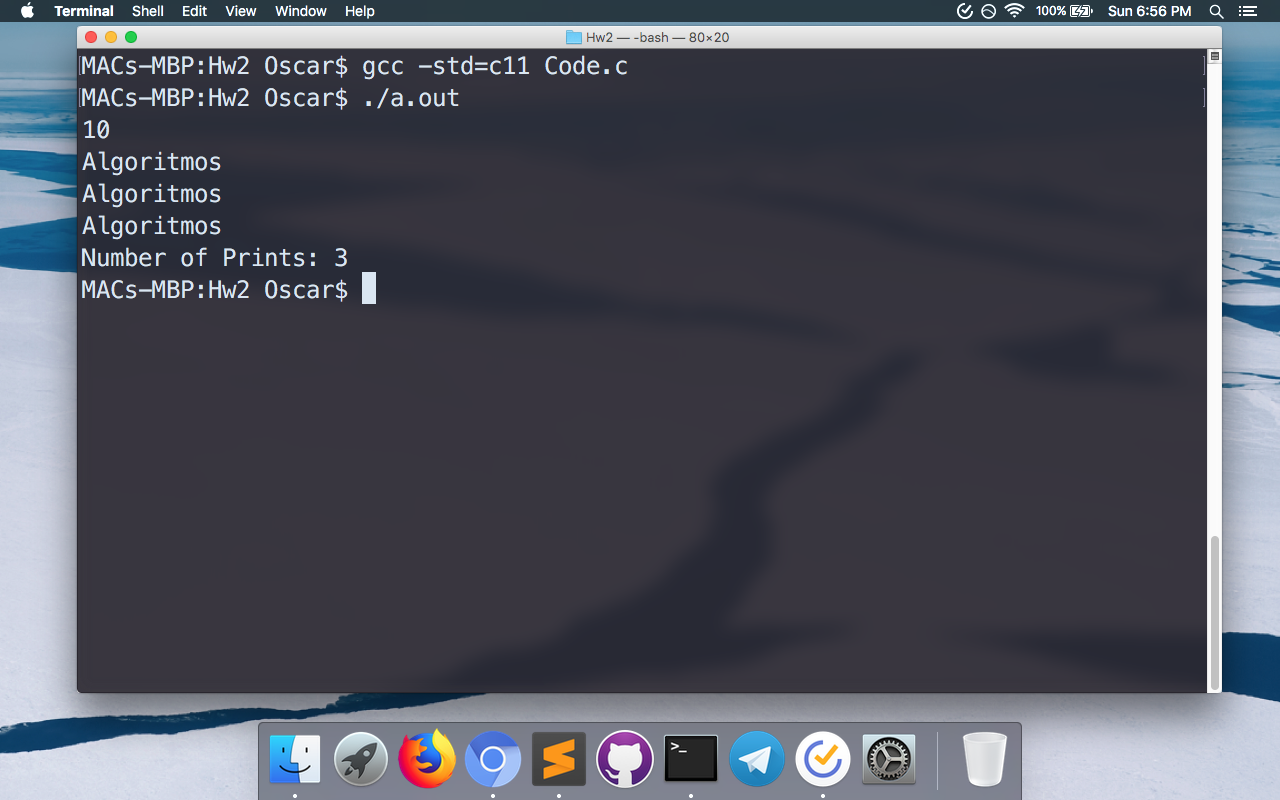
\includegraphics[width=0.45\textwidth]{6-1}
            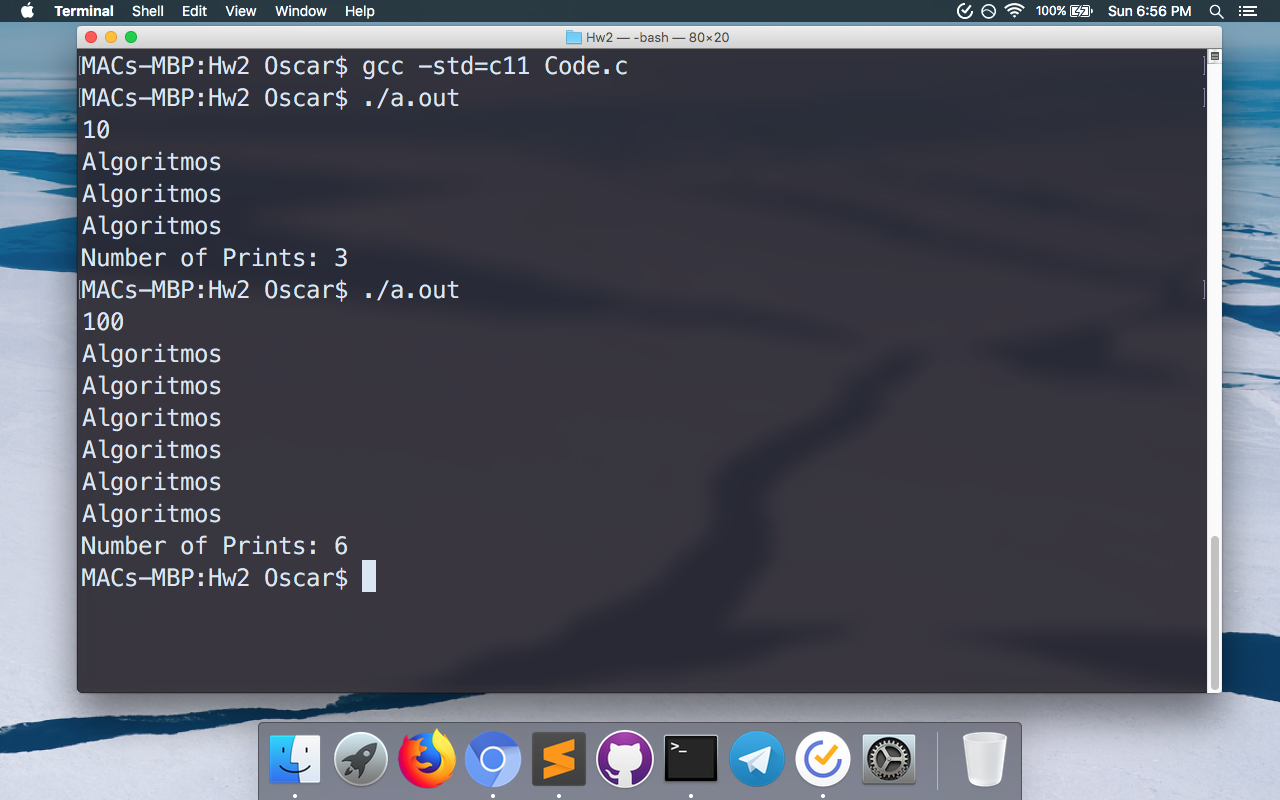
\includegraphics[width=0.45\textwidth]{6-2}
            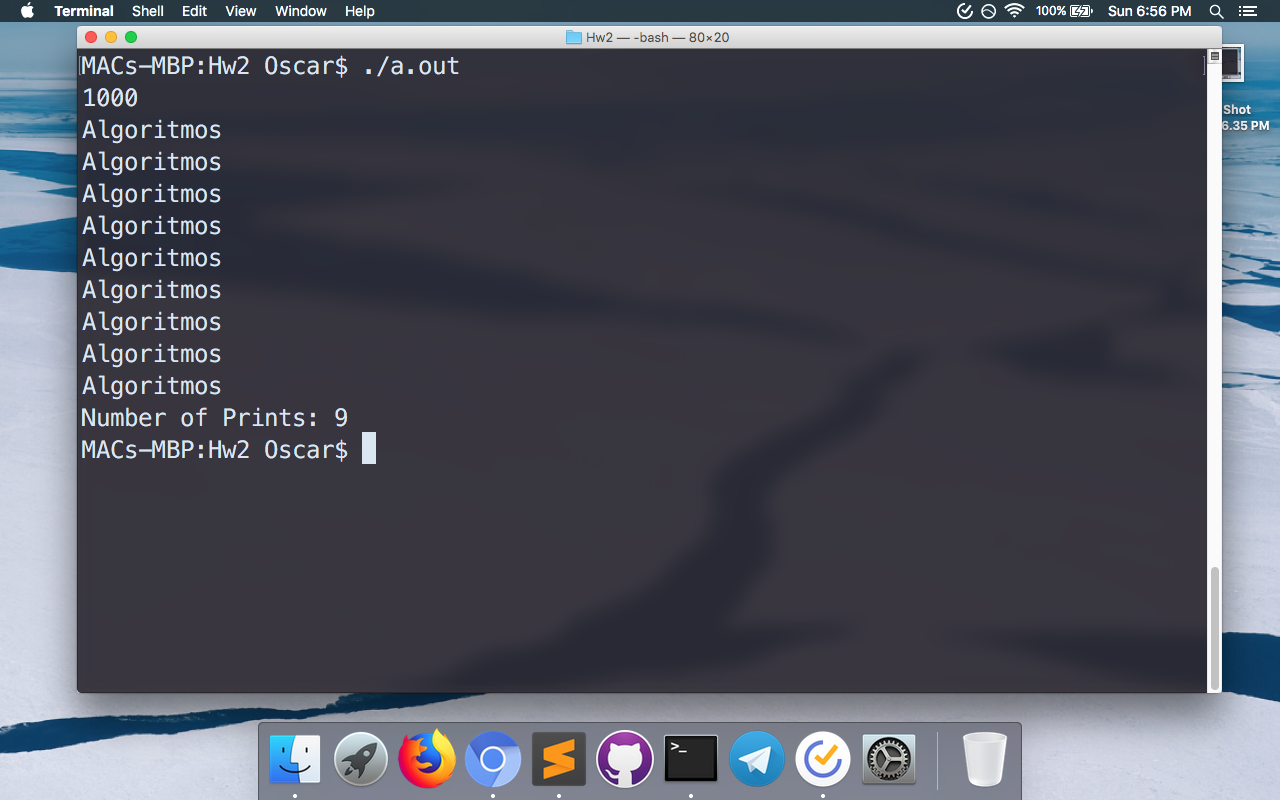
\includegraphics[width=0.45\textwidth]{6-3}
            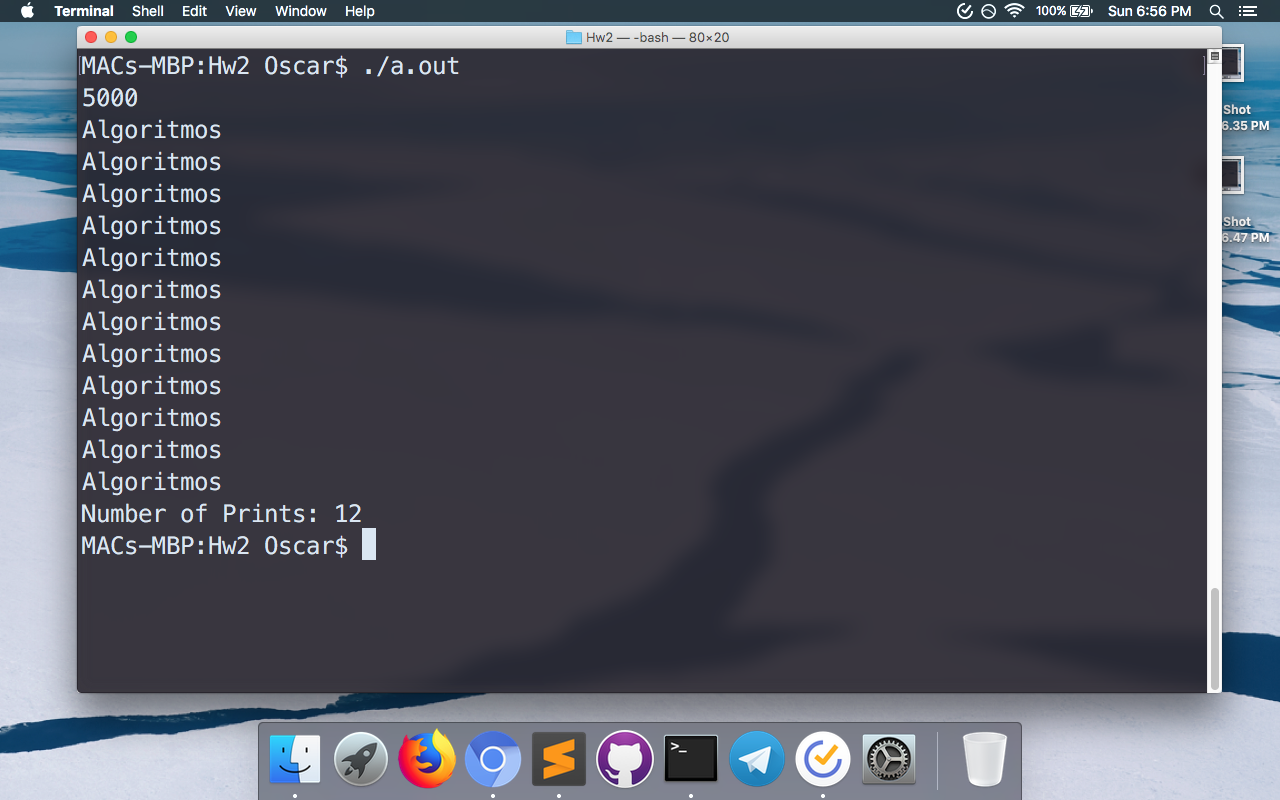
\includegraphics[width=0.45\textwidth]{6-4}
            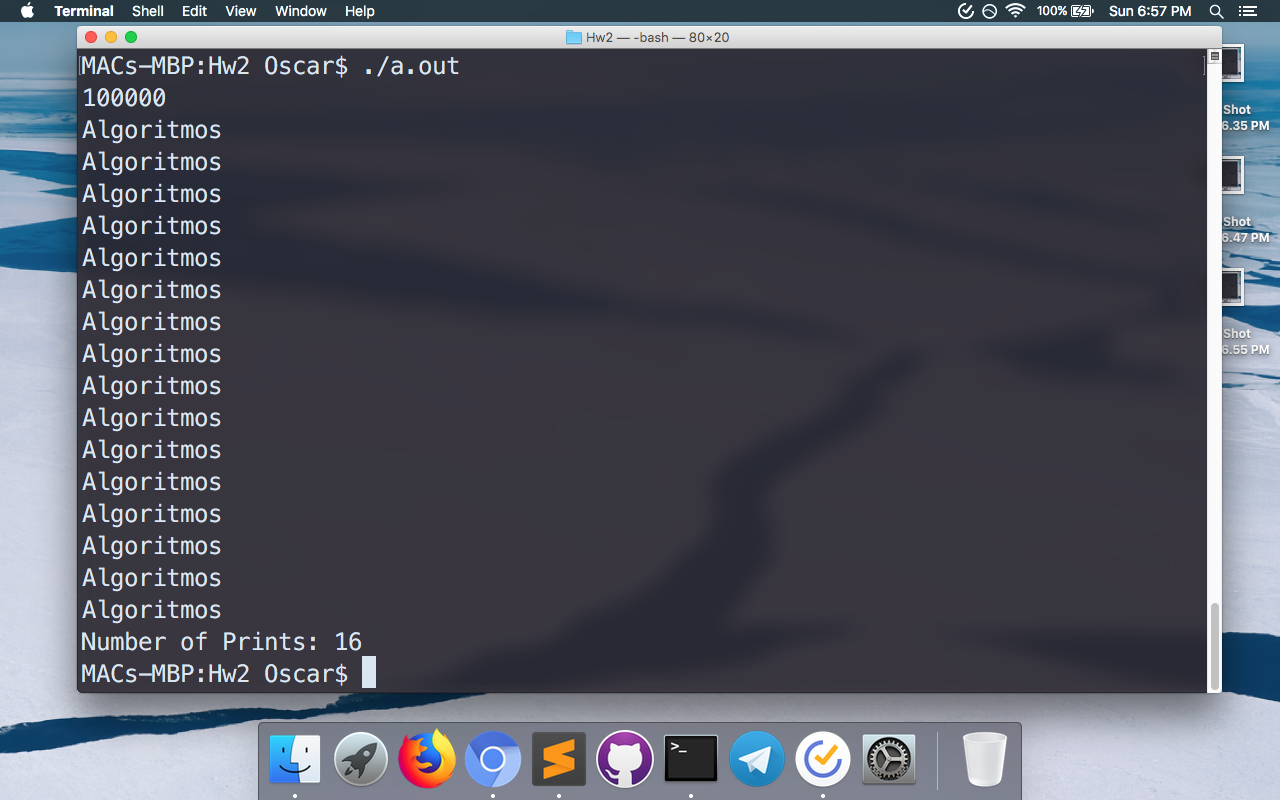
\includegraphics[width=0.45\textwidth]{6-5}
        \end{figure}

    \end{SmallIndentation}


    % ============================================================
    % =================          ALGORITMOS      =================
    % ============================================================
    \clearpage
    \subsection{Algoritmo 7}
    \begin{SmallIndentation}[0em]

        Considera el siguiente algoritmos
        \begin{lstlisting}[language=C, gobble=12, basicstyle=\small\color{white}]
            #include <stdio.h>

            int main() {
                int n;
                scanf("%d", &n);

                int NumberOfPrints = 0;
                
                for(int j = n / 2; j > 1; j /= 2) {
                    for(int i = 0; i < n; i += 2) {
                        //printf("\"Algoritmos\"\n");
                        count++;
                    }
                }

                printf("Number of Prints: %d\n", NumberOfPrints);
                return 0;
            }
        \end{lstlisting}


        \begin{enumerate}

            \item Vamos primero por el for generico interno:
                $NumInnerFor 
                    = \Floor{\frac{End - Start}{Jump} + 1}
                    = \Floor{\frac{n - 1 - 0}{2} + 1}
                    = \Floor{\frac{n}{2}}$


            \item
                Ahora podemos calcular del for exterior, lo cual tenemos que:

                $NumInnerFor 
                    = \Floor{\log_{Jump}\pfrac{End}{Start} + 1}
                    = \Floor{\log_{2}\pfrac{\frac{n}{2}}{2}}$
        \end{enumerate}

        Finalmente tenemos que Numero de Prints $ = Floor{\frac{n}{2}}\Floor{\log_{2}\pfrac{\frac{n}{2}}{2}}$
            


        Ahora vamos a resolver para algunas $n$ y veamos como se compara con
        la realidad:

        \begin{tabular}{r ||c |c | c |c }
            % And this is the name of all the headers
            &  Numero de N & Resultado Real & Resultado Teorico & \\ [0.5ex] 
            \hline\hline
          
            %Body
            & 10 &  5 &
                $\Floor{\frac{10}{2}}\Floor{\log_{2}\pfrac{\frac{10}{2}}{2}}
                    = 5 \Floor{\log_{2}(2.5)}
                    = 5 \Floor{1.32} = 5$
                    &  \\[0.6cm]
            & 100 &  200 &
                $\Floor{\frac{100}{2}}\Floor{\log_{2}\pfrac{\frac{100}{2}}{2}}
                    = 50 \Floor{\log_{2}(25)}
                    = 50 \Floor{4.64} = 200$
                    &  \\[0.6cm]
            & 1000 &  3500 &
                $\Floor{\frac{1000}{2}}\Floor{\log_{2}\pfrac{\frac{1000}{2}}{2}}
                    = 500 \Floor{\log_{2}(250)}
                    = 500 \Floor{7.96} = 3500$
                    &  \\[0.6cm]
            & 5000 &  25000 &
                $\Floor{\frac{5000}{2}}\Floor{\log_{2}\pfrac{\frac{5000}{2}}{2}}
                    = 2500 \Floor{\log_{2}(1250)}
                    = 2500 \Floor{10.28} = 25000$
                    &  \\[0.6cm]
            & 100000 &  700000 &
                $\Floor{\frac{100000}{2}}\Floor{\log_{2}\pfrac{\frac{100000}{2}}{2}}
                    = 50000 \Floor{\log_{2}(14.609)}
                    = 50000 \Floor{14.609} = 700000$
                    &  \\[0.6cm]
        \end{tabular}

        \clearpage


        % =====================================================
        % ============    SPACE FOR JUST IMAGE     ============
        % =====================================================
        
        Vamos a mostar ahora las evidencias:
        
        \begin{figure}[h]
            \centering
            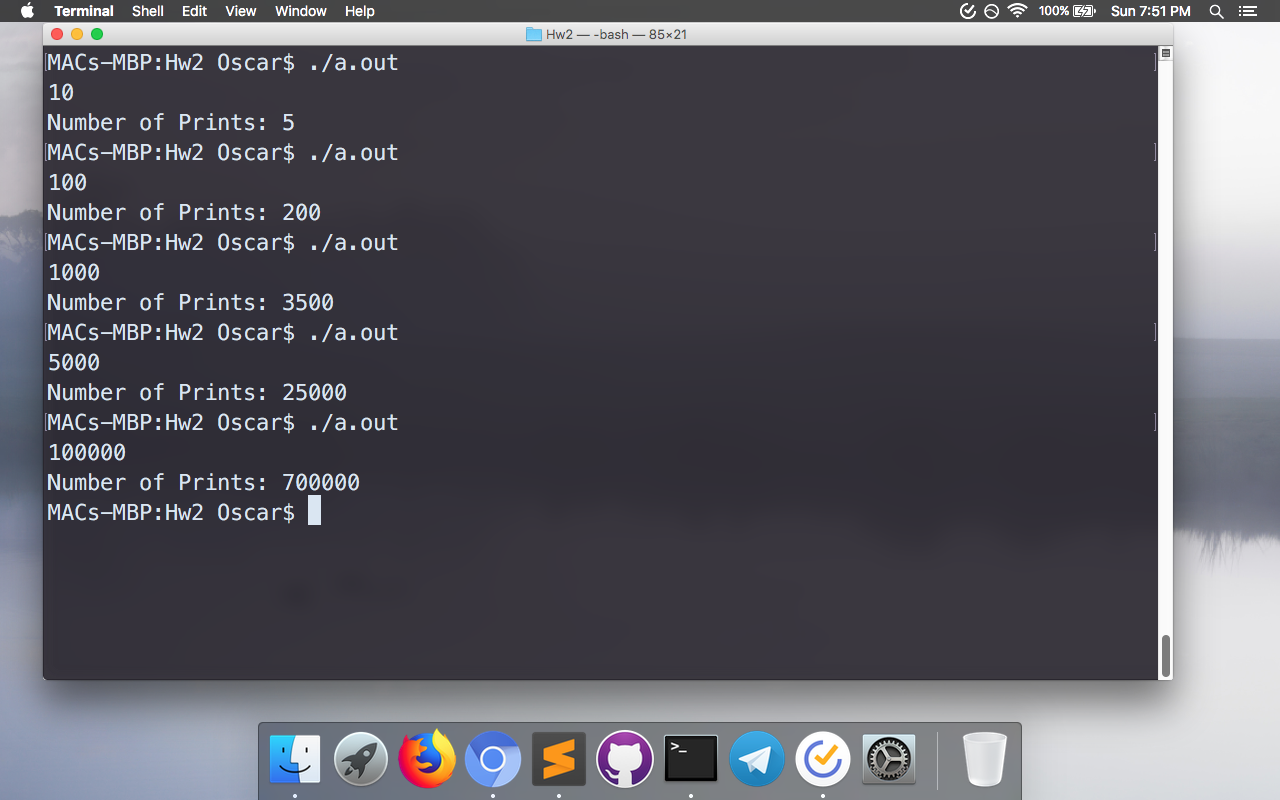
\includegraphics[width=0.85\textwidth]{7}
        \end{figure}

    \end{SmallIndentation}
            
    % ============================================================
    % =================          ALGORITMOS      =================
    % ============================================================
    \clearpage
    \subsection{Algoritmo 8}
    \begin{SmallIndentation}[0em]

        Considera el siguiente algoritmos
        \begin{lstlisting}[language=C, gobble=12, basicstyle=\small\color{white}]
            #include <stdio.h>

            int main() {
                int n;
                scanf("%d", &n);

                int NumberOfPrints = 0;
                int i = n:

                while(i >= 0){
                    for(int j = n; i < j; i -= 2, j /= 2){
                        //printf("Algoritmos\n");
                        NumberOfPrints++;
                    }
                }

                printf("Number of Prints: %d\n", NumberOfPrints);
                return 0;
            }
        \end{lstlisting}


        Esta es muy curiosa porque se cicla, ya que al entrar a while $i = n$, 
        pero nunca vamos a entrar al for, pues la condición es que $i < j$, pero
        en el momento de la primera comparación $ i = j$, por lo tanto
        se va a quedar ahi, dentro del while, para siempre.
    \end{SmallIndentation}
            







% ============================================================
% ========     APROXIMACION DE NUMERO DE PRINTS     ==========
% ============================================================
\clearpage
\section{Análisis de Casos de Prints}

    Para los siguientes algoritmos determine las funciones de complejidad
    temporal, para el mejor caso, peor caso y caso medio. Indique cual(es)
    son las condiciones (instancia de entrada) del peor caso y cual(es) la del
    mejor caso.


    % ============================================================
    % =================          ALGORITMOS      =================
    % ============================================================
    \clearpage
    \subsection{Algoritmo 9}

        Considera el siguiente algoritmos
        \begin{lstlisting}[language=C, gobble=12, basicstyle=\small\color{white}]
            func Producto2Mayores(A,n)
                if(A[1] > A[2])
                    mayor1 = A[1];
                    mayor2 = A[2];
                else
                    mayor1 = A[2];
                    mayor2 = A[1];
                
                i = 3;

                while(i <= n)
                    if(A[i] > mayor1)
                    mayor2 = mayor1;
                    mayor1 = A[i];
                    else if (A[i] > mayor2)
                    mayor2 = A[i];
                    i = i + 1;

                return mayor1 * mayor2;
        \end{lstlisting}

        Usaremos las recomendaciónes, es decir
        usamos como operaciones básicas:
        comparación entre elementos del arreglo A y
        Asignaciones a mayor1 y mayor 2.


        % ============================================================
        % ================     MEJOR CASO      =======================
        % ============================================================
        \vspace{1em}
        \subsubsection{Mejor Caso}

            Ok, en este caso es sencilla, al ser una modificación de una busqueda lineal
            es fácil encontrar el mejor caso.

            Este se da cuando el elemento mayor de A es A[1] y el siguiente mayor es A[2].

            Porque entonces son solo 3 operaciones que se ejecutan antes del while, mientras
            que el while simplemente se ejecutan $2(n-2)$, entonces nota que:
            el mejor caso es $f(n) = 2n + 1$


        % ============================================================
        % ================      PEOR CASO      =======================
        % ============================================================
        \clearpage
        \subsubsection{Peor Caso}

            Ok, en este caso es sencilla, al ser una modificación de una busqueda lineal
            es fácil encontrar el peor caso.

            Este se da cuando el arreglo este ordenado de menor a mayor, porque en ese caso
            se hara:
            \begin{itemize}
                \item 3 instrucciones antes del while
                \item n-2 veces:
                    \item 3 veces al cumplirse el primer if
            \end{itemize}

            Por lo tanto tenemos que el peor caso esta dado por:
            $f(n) = 3n - 3$


        % ============================================================
        % ================      PEOR CASO      =======================
        % ============================================================
        \vspace{1em}
        \subsubsection{Caso Medio}

            Ok, en este caso es díficil, por un lado tenemos que arriba del while
            sin importar que pasa se ejecutan 3 instrucciones, pero pero adentro del
            while pasan cosas raras:
            \begin{itemize}
                \item $\frac{1}{3}$ de las veces en promedio se ejecuta el primer if, es 
                    decir $3n - 3$
                \item $\frac{1}{3}$ de las veces en promedio se ejecuta el segundo if, es 
                    decir $3n - 3$
                \item $\frac{1}{3}$ de las veces en promedio no se ejecuta nada, es 
                    decir $2n - 1$
            \end{itemize}

            Por lo tanto tenemos que el peor caso esta dado por:
            $f(n) = 3 + \frac{1}{3}(3n-3)+ + \frac{1}{3}(3n-3) + + \frac{1}{3}(2n-1) = \frac{8 - 7}{3}n$



    % ============================================================
    % =================          ALGORITMOS      =================
    % ============================================================
    \clearpage
    \subsection{Algoritmo 10}

        Considera el siguiente algoritmos
        \begin{lstlisting}[language=C, gobble=12, basicstyle=\small\color{white}]
            func OrdenamientoIntercambio(a, n)
            for (i = 0; i < n - 1; i++)              
                for (int j = i + 1; j < n; j++)      
                    if (a[j] < a[i]) {                
                        temp = a[i];
                        a[i] = a[j];
                        a[j] = temp;
                    }                               
        \end{lstlisting}

        Usaremos las recomendaciónes, es decir
        usamos como operaciones básicas:
        comparación entre elementos del arreglo a y
        Asignaciones a temp y al arreglo a.


        % ============================================================
        % ================     MEJOR CASO      =======================
        % ============================================================
        \subsubsection{Mejor Caso}

            No podemos hacer nada para evitar la ejecucción de los dos
            fors, pero si que podemos evitar la ejecucción de todas
            las instrucciones dentro del if, por lo tanto
            el mejor caso es simplemente cuando el arreglo esta ordenado de menor a mayor.

            Ahora, vemos que la función se puede sacar facilmente como:
            \begin{itemize}
                \item El for interno se ejecuta cada $n-1 - i + 1$ veces, mas sencillo
                es $n - i$ veces
                \item Ahora vamos a ver cuantas veces se ejecuta el for de afuera, es sencillo
                pues son $(n-1)$ veces 
            \end{itemize}

            Por lo tanto su suma es sencillamente $\frac{n^2 - n}{2}$


        % ============================================================
        % ================      PEOR CASO      =======================
        % ============================================================
        \subsubsection{Peor Caso}

            Ok, ahora que vimos el mejor caso, el peor caso es muy sencillo, es cuando
            el arreglo esta ordenado de mayor a menor y es porque siempre, siempre
            se van a ejecutar las instrucciones del if, es decir, 4 veces mas que antes
            por lo tanto es tan sencillo calcularlo como:
            $f(n) = 4 \frac{n^2 - n}{2} = 2n^2 - 2n$


        % ============================================================
        % ================      PEOR CASO      =======================
        % ============================================================
        \subsubsection{Caso Medio}

            Ahora esta esta sencilla, pero engañosa, y es que existe la misma posibilidad
            de que se ejecute el if o no, por lo tanto y SOLO EN ESTE CASO el caso
            promedio se puede aproximar usando el promedio del mejor y menor, es
            decir $f(n) = \frac{5n^2 - 5n}{2}$




    % ============================================================
    % =================          ALGORITMOS      =================
    % ============================================================
    \clearpage
    \subsection{Algoritmo 11}

        Considera el siguiente algoritmos
        \begin{lstlisting}[language=C, gobble=12, basicstyle=\small\color{white}]
            func MaximoComunDivisor(m, n){
                a = max(n, m);
                b = min(n, m);
                residuo = 1;
                mientras (b > 0){
                    residuo = a mod b;
                    a = b;
                    b = residuo;
                }
                MaximoComunDivisor = a;
                return MaximoComunDivisor;
            }                            
        \end{lstlisting}

        Usaremos las recomendaciónes, es decir usamos como operaciones básicas:
        operaciones básicas y la operación de modulo de a y b


        % ============================================================
        % ================     MEJOR CASO      =======================
        % ============================================================
        \subsubsection{Mejor Caso}

            Ok, voy a ser un poco tramposo, pero el mejor caso sería cuando $n = 0$
            en ese caso nunca entramos al while y por lo tanto es cero.

            Es bastante obvio que otro caso bastante bueno es cuando $ m = kn$ es decir
            que uno es multiplo de otro, pero nada supera a ese caso.


        % ============================================================
        % ================      PEOR CASO      =======================
        % ============================================================
        \subsubsection{Peor Caso}


            Ok, tengo que admitir que este es un problema conocido, es el clásico algoritmo de Euclides
            y hay un caso muy feo para ese algoritmo, y es que sean dos número de Fibonacci consecutivos.

            Vamos a dar una explicación de porque:
            Por definición $F_{k} = F_{k -1} + F_{k - 2}$, por lo tanto cuanto lo divides tienes que 
            que el cociente siempre sera 1 en cada iteración, por lo tanto tardaremos $k$ divisiones en 
            llegar a $k$, y como los números de Fibonacci se aproximan a $\phi^k$ entonces
            tenemos que el peor caso será $f(n) = \log{\phi}(n)$



        % ============================================================
        % ================      PEOR CASO      =======================
        % ============================================================
        \subsubsection{Caso Medio}

            Si no son el peor caso entonces el cociente nunca podrá ser 1, es decir en cada paso podremos
            dividir a la mitad el mayor número por lo tanto, es lo inverso a una exponcial es sencillo deducir
            que es $f(n) = \log_2(n)$



    % ============================================================
    % =================          ALGORITMOS      =================
    % ============================================================
    \clearpage
    \subsection{Algoritmo 12}

        Considera el siguiente algoritmos
        \begin{lstlisting}[language=C, gobble=12, basicstyle=\small\color{white}]
            func BurbujaOptimizada(A, n)
                cambios = "Si"
                i = 0
                Mientras i < n - 1 && cambios != "No" hacer 
                    cambios = "No"
                    Para j = 0 hasta (n - 2) - i hacer
                        Si A[j + 1] < A[j] hacer    
                            aux = A[j]
                            A[j] = A[j + 1]
                            A[j + 1] = aux
                            cambios = "Si"
                        Fin Si             
                    Fin Para
                    i = i + 1
                Fin Mientras
            Fin func
        \end{lstlisting}

        Usaremos las recomendaciónes, las comparaciones entre elementos del arreglo A, asignaciones
        a aux y al arreglo A.

        % ============================================================
        % ================     MEJOR CASO      =======================
        % ============================================================
        \subsubsection{Mejor Caso}

            Ok, esta también esta sencilla, no puedes hacer nada para cambiar el flow del programa
            mas que evitando entrar en los ifs, así como al while, por lo tanto si nuestro array
            esta ordenado, en cuyo cas tenemos que $n - 1$


        % ============================================================
        % ================      PEOR CASO      =======================
        % ============================================================
        \subsubsection{Peor Caso}


            Es lo inverso, es cuando siempre entramos en el while y siempre en el if, por lo tanto
            es lo inverso, cuando esta ordenado pero de mayor a menor.

            Por lo tanto:
            \begin{align*}
                f(n)
                    &= \sum_{i = 0}^{n - 2} \sum_{i = 0}^{n - 2 - i} 4      \\
                    &= 4(n-1)(n-1) - \frac{4(n-1)(n-1)}{2}                  \\
                    &= 2n^2 - 2n 
            \end{align*}



        % ============================================================
        % ================      PEOR CASO      =======================
        % ============================================================
        \subsubsection{Caso Medio}

            De forma similar tenemos dos bifuraciones con el if, suponiendo que tenemos la misma
            probabilidad de entrar es sencillo ver que:
            $f(n) = \frac{5n^2 - 5n}{2}$



    % ============================================================
    % =================          ALGORITMOS      =================
    % ============================================================
    \clearpage
    \subsection{Algoritmo 13}

        Considera el siguiente algoritmos
        \begin{lstlisting}[language=C, gobble=12, basicstyle=\small\color{white}]
            func BurbujaSimple(A, n)
                Para i = 0 hasta n - 2 hacer            
                    Para j = 0 hasta (n - 2) - i hacer  
                        Si A[j + 1] < A[j] hacer        
                            aux = A[j]
                            A[j] = A[j + 1]
                            A[j + 1] = aux
                        Fin Si                          
                    Fin Para
                Fin Para
            Fin func
        \end{lstlisting}

        Usaremos las recomendaciónes, las comparaciones entre elementos del arreglo A, asignaciones
        a aux y al arreglo A.

        % ============================================================
        % ================     MEJOR CASO      =======================
        % ============================================================
        \subsubsection{Mejor Caso}

            Ok, esta también esta sencilla, no puedes hacer nada para cambiar el flow del programa
            mas que evitando entrar en los ifs, así como al while.
            Por lo tanto lo mejor que nos puede pasar es que el arreglo ya este ordenado ascendentemente

            Ahora, vemos que la función se puede sacar facilmente como:
            \begin{itemize}
                \item El for interno se ejecuta cada $n-1 - i + 1$ veces, mas sencillo
                es $n - i$ veces
                \item Ahora vamos a ver cuantas veces se ejecuta el for de afuera, es sencillo
                pues son $(n-1)$ veces 
            \end{itemize}

            Por lo tanto su suma es sencillamente $\frac{n^2 - n}{2}$



        % ============================================================
        % ================      PEOR CASO      =======================
        % ============================================================
        \subsubsection{Peor Caso}


            Es lo inverso, es cuando siempre entramos en el while y siempre en el if, por lo tanto
            es lo inverso, cuando esta ordenado pero de mayor a menor.

            Por lo tanto:
            \begin{align*}
                f(n)
                    &= \sum_{i = 0}^{n - 2} \sum_{i = 0}^{n - 2 - i} 4      \\
                    &= 4(n-1)(n-1) - \frac{4(n-1)(n-1)}{2}                  \\
                    &= 2n^2 - 2n 
            \end{align*}



        % ============================================================
        % ================      PEOR CASO      =======================
        % ============================================================
        \subsubsection{Caso Medio}

            De forma similar tenemos dos bifuraciones con el if, suponiendo que tenemos la misma
            probabilidad de entrar es sencillo ver que:
            $f(n) = \frac{5n^2 - 5n}{2}$




    % ============================================================
    % =================          ALGORITMOS      =================
    % ============================================================
    \clearpage
    \subsection{Algoritmo 14}

        Considera el siguiente algoritmos
        \begin{lstlisting}[language=C, gobble=12, basicstyle=\small\color{white}]
            func Ordena(a, b, c)
                if(a > b)
                    if(a > c)
                        if(b > c)
                            salida(a, b, c);        
                        else
                            salida(a, c, b);       
                    else
                        salida(c, a, b);           
                else
                    if(b > c)
                        if(a > c)
                            salida(b, a, c);        
                        else
                            salida(b, c, a);        
                    else
                        salida(c, b, a);           
            Fin func
        \end{lstlisting}

        Usaremos las recomendaciónes, las comparaciones entre a, b, c.

        Ok, voy a analizar este problema un poco diferente, porque voy a ir a cada camino posible
        como no son muchos contando las comparaciones:
        \begin{lstlisting}[language=C, gobble=12, basicstyle=\small\color{white}]
            func Ordena(a, b, c)
                if(a > b)
                    if(a > c)
                        if(b > c)
                            salida(a, b, c);        // 3 Operaciones  
                        else
                            salida(a, c, b);        // 3 Operaciones        
                    else
                        salida(c, a, b);            // 2 Operaciones  
                else
                    if(b > c)
                        if(a > c)
                            salida(b, a, c);        // 3 Operaciones
                        else
                            salida(b, c, a);        // 3 Operaciones
                    else
                        salida(c, b, a);            // 2 Operaciones
            Fin func
        \end{lstlisting}

        % ============================================================
        % ================     MEJOR CASO      =======================
        % ============================================================
        \subsubsection{Mejor Caso}

            Ok, este problema esta sencillo de analizar por la falta de ciclos raros y feos,
            esto ayuda mucho.

            Entonces, lo mejor que nos prodria pasar es entrar al primer if, y al segundo ... y al
            tercero, es decir cuando $a > b$ y $a \leq c$.

            O bien, igualmente cuando $a \leq b$ y $b \leq c$

            Con $f(n) = 2$



        % ============================================================
        % ================      PEOR CASO      =======================
        % ============================================================
        \subsubsection{Peor Caso}


            Es lo inverso, y pasa que como este algoritmo solo puede tardar 2 tiempos diferentes
            entonces el peor caso es cualquier entrada que no sea el mejor caso.



        % ============================================================
        % ================      PEOR CASO      =======================
        % ============================================================
        \subsubsection{Caso Medio}

            Por primera vez creo que hare una función que si sea realmente la correcta, es decir
            es cada uno de los tiempos por la probabilidad de que ocurra, es decir:
            $f(n) = \frac{4}{6}(2) + \frac{2}{6}(3) = \frac{8}{3}$




    % ============================================================
    % =================          ALGORITMOS      =================
    % ============================================================
    \clearpage
    \subsection{Algoritmo 15}

        Considera el siguiente algoritmos
        \begin{lstlisting}[language=C, gobble=12, basicstyle=\small\color{white}]
            func Seleccion(A, n)
                Para k = 0 hasta n - 2 hacer            
                    p = k
                    Para i = k + 1 hasta n - 1 hacer    
                        Si A[i] < A[p] entonces         
                            p = i
                        Fin Si                          
                    Fin Para
                    temp = A[p]
                    A[p] = A[k]
                    A[k] = temp                         
                Fin Para
            Fin func
        \end{lstlisting}

        Usaremos como operaciones basicas las comparaciones entre elementos del arreglo A, asignaciones
        a temp y al arreglo A.

        % ============================================================
        % ================     MEJOR CASO      =======================
        % ============================================================
        \subsubsection{Mejor Caso}

            Como ya va siendo costumbre en el mejor caso en los algoritmos de ordenamiento es que
            este ordenado ascendentemente,porque en ese caso nunca entramos a los if, por lo tanto 
            podemos encontrar la función facilmente gracias a las operaciones que estamos contando:
            \begin{align*}
                f(n)
                    &= \sum_{k = 0}^{n-2} \Wrap{3 + \sum_{i = k +1}^{n-1} 1}    
                    &&= \sum_{k = 0}^{n-2} 3 + n  - 1 + k                        \\
                    &= \frac{2n^2 + 2n - 4 - n^2+ 3n -2}{2}                     
                    &&= \frac{n^2 + 5n - 6}{2}
            \end{align*}



        % ============================================================
        % ================      PEOR CASO      =======================
        % ============================================================
        \subsubsection{Peor Caso}


            Es lo inverso, y pasa que como este algoritmo incluso si entra dentro del if  y en 
            la vida real si que se tardaría mas como no estamos contando eso como una operación resulta
            que el valor es igual:
            $f(n) = \frac{n^2 + 5n - 6}{2}$



        % ============================================================
        % ================      PEOR CASO      =======================
        % ============================================================
        \subsubsection{Caso Medio}

            Jajaja, ahora esto esta sencillo, porque si su caso mejor y peor son el mismo adivina cual es su
            caso medio $f(n) = \frac{n^2 + 5n - 6}{2}$



\end{document}